%\documentclass[12pt,a4paper,twoside]{article}
\documentclass[a4paper,twoside]{llncs}
\usepackage[utf8]{inputenc}
\usepackage{amsmath,amsfonts,amssymb}
\usepackage{graphicx}
\usepackage{algorithmic,algorithm}
\usepackage{tikz}
\usetikzlibrary{matrix,arrows,decorations.pathmorphing,shapes,snakes}

\pagestyle{headings}%page numbers

%%%%%%%%%%%%%%%%%%%%%%%%%%% VERSIONES %%%%%%%%%%%%%%%%%%%%%%%%%%%%%%%%%%%
\newcommand{\version}{Versi\'on 0.0.1}
%%%%%%%%%%%%%%%%%%%%%%%%%%%%%%%%%%%%%%%%%%%%%%%%%%%%%%%%%%%%%%%%%%%%%%%%%

\title{Generalised Rijndael}
\author{Sergi Blanch-Torn\'e\inst{1}, Ramiro Moreno Chiral\inst{2}, Francesc Seb\'e Feixa\inst{2}}
 \institute{
 Escola Polit\`ecnica Superior, Universitat de Lleida. Spain.\\
 \email{\tt sblanch@alumnes.udl.es}
 \and 
 Departament de Matem\`atica. Universitat de Lleida. Spain.\\
 \email{\tt \{ramiro,fsebe\}@matematica.udl.es}
 }

%%% abreviaturas matem\'aticas
% Enteros
\newcommand{\Z}{\ensuremath{\mathbb{Z}}} 

% Anillo de los enteros mod n
\newcommand{\Zn}[1]{\ensuremath{\mathbb{Z}/#1\mathbb{Z}}} 

% Cuerpo finito de orden p (primo)
\newcommand{\Fq}[1]{\ensuremath{\mathbb{F}_#1}} 

% Cuerpo finito de caractar\'{\i}stica p, grado n
\newcommand{\Fpn}[2]{\ensuremath{\mathbb{F}_{#1^#2}}} 

% Anillo polinomial con coeficientes en un cuerpo polinomial binario
\newcommand{\Fpnm}[2]{\ensuremath{\frac{\Fpn{2}{#1}[#2]}{m(#2)}}}

\renewcommand{\algorithmicrequire}{\textbf{INPUT:}}%
\renewcommand{\algorithmicensure}{\textbf{OUTPUT:}}%
\renewcommand{\algorithmiccomment}[1]{/* #1 */}%	

%used for schemas
\newcommand{\myunit}{1 cm}
\tikzset{
    node style sp/.style={draw,circle,minimum size=\myunit},
    node style ge/.style={circle,minimum size=\myunit},
    arrow style mul/.style={draw,sloped,midway,fill=white},
    arrow style plus/.style={midway,sloped,fill=white},
}

\floatname{algorithm}{Algorithm}%
\floatname{definition}{Definition}%

\begin{document}
\maketitle
\begin{center}
 \today\\
 \version
\end{center}

\begin{abstract}\footnote{Partially founded by the Spanish project MTM20\_\_-\_\_\_\_\_-\_\_\_-\_\_}
 This is the abstract
% TODO this article comes from a real request, for small block cipher, but the tuneable paramenters in rijndael creates the idea to, further than an small version, it can be generalized
\\\\    
{\bf Keywords:} Cryptography, Symmetrics, Rijndael
\end{abstract}

%%%%%%%%%%%%%%%%
\section{Introduction}
% TODO There are many other options of symmetric ciphers with different block sizes. AES is very static, but rijndael allows to play with paramenters. AESwrap (rfc3394) can be mention as another possibility.
% TODO problem aproach (rijndael scalability)
% TODO alternative cryptosystems

\cite{Daemen:1998:BCR:646692.759487}
\cite{Daemen98aesproposal:}
\cite{rfc3394}
\cite{AES-FIPS}


%%%%%%%%%%%%%%%%
\section{Approach to the Rijndael Schema}
% what is a PRP? 
\begin{definition}\label{def:PRP}
 A Pseudo-Random Permutation (PRP) is defined as a application from the message space $\mathcal{M}$ and the key space $\mathcal{K}$ to the cipher space $\mathcal{C}$:
 \begin{center}
  \begin{tabular}{llll}
   PRP: & $\mathcal{M} \times \mathcal{K}$ & $\rightarrow$ & $\mathcal{C}$ \\
  \end{tabular}
 \end{center}
 such that:
 \begin{enumerate}
  \item $\exists$ ``efficient'' \emph{deterministic} algorithm $c=E(k,m)$
  \item The functions $E$ is bijective
  \item $\exists$ ``efficient'' inversion algorithm such that $m=D(k,c)$
 \end{enumerate}
\end{definition}

A pseudo-random permutation is used as a symmetric cryptosystem like Shannon have defined in \cite{shannon-comTheorySecSys}. Also Shannon have defined the concept of the \emph{perfect secrecy}
\begin{definition}
 A \emph{cipher} has \emph{perfect secrecy} if $\forall m_1, m_2 \in \mathcal{M} \;s.t.\; \left| m_1 \right| = \left| m_2 \right| \wedge \forall c \in \mathcal{C}$ and a $k\in_R\mathcal{K}$ (random and uniform distributed), the probability to that $c$ comes from $m_1$ or $m_2$ are the same
 \begin{center}
  $Pr[E(k,m_1)=c] = Pr[E(k,m_2)=c]$
 \end{center}
\end{definition}

This means that $c$ does not reveal \emph{any} information about the originam $m$. This can also by says like: The distribution of the cipher of a message is the same than the distribution from another message, or formally:
\begin{definition}
 For a perfect secrecy system, the distributions of the ciphers between messages in the cipher space is computationally indistinguishable:
 \begin{center}
  $\{ E(k,m_1) \} \approx_p \{ E(k,m_2) \} $
 \end{center}
\end{definition}

Consider an scenario where an adversary has access to a random oracle where the output of this oracle can be or the output of the PRP or a truly random output, the advantage of the adversary to distinguish between if the output is get from one or the other can be described as:
\begin{equation}\label{eq:prpAdv}
 {Adv}_{F}^{prp}(A) = Pr[{Exp}_{F}^{prp-1}(A)=1]-Pr[{Exp}_{F}^{prp-0}(A)=1]
\end{equation}
where ${Exp}_{F}^{PRP-1}$ is the probability to the adversary to win the bet that the output comes from a the PRP and ${Exp}_{F}^{PRP-0}$ when the output comes from a truly random.

\begin{definition}\label{def:securePRP}
 A PRP is secure if for all ``efficient'' adversary, the advantage to distinguish if the output is from the PRP or the truly random is ``negligible''
\end{definition}
% TODO and why is Rijndael a secure PRP?
The most efficient attacks on Rijndael      that means this algorithm is still secure.

% TODO rijndael good characteristics
% TODO shannon: confusion & diffusion => substitution & permitation
% TODO structure of the input (fix block size)
% TODO format preserving encryption alternative?

%%%%%%%%%%%%%%%%
\subsection{Design}
% TODO what is the state matrix
% TODO describe the transformations from the Shammir ``confussion and diffusion'' point of view.

%%%%%%%%%%%%%%%%
\section{Generalising the schema}

% Draw the procedure as diagram
\begin{figure}[h]
 \centering
 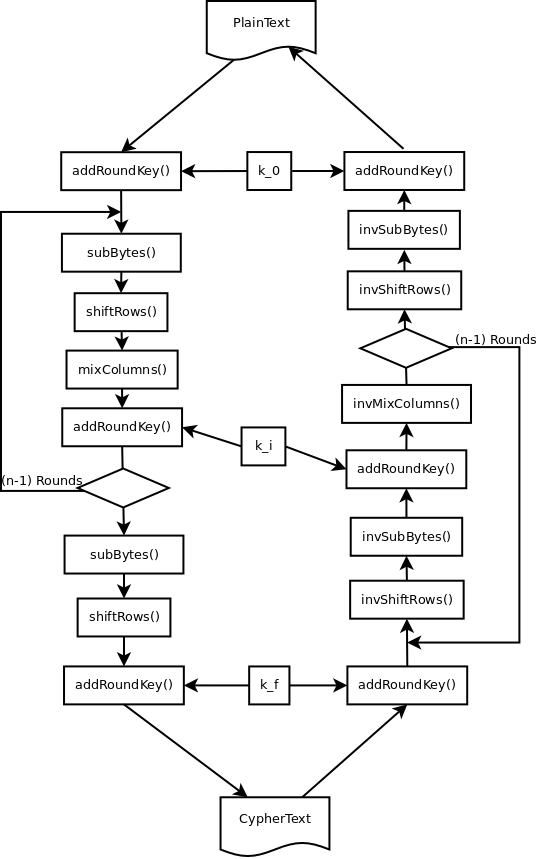
\includegraphics[scale=0.3,keepaspectratio=true]{./images/rijndaelDiagram.png}
 % rijndaelDiagram.png: 521x887 pixel, 72dpi, 18.38x31.29 cm, bb=0 0 521 887
 \caption{rijndael diagram}
 \label{fig:RijndaelDiagram}
\end{figure}
% TODO 

%%%%%%%%%%%%%%%%
\subsection{key expansion}
% TODO define s Pseudo-Random Generator (PRG)
% TODO abstraction of what it is, independent from the #rows, #columns, wordsize
% TODO subBytes() is used, then the sboxes but is explained later on.
% TODO when key n#columns is different than message #columns

\begin{algorithm}
 \caption{KeyExpansion}
 \label{alg:keyExpansion}
 \begin{algorithmic}[1]
  \REQUIRE byte k[nRows*nColumns], nRounds, nRowns, nColumns, wSize
  \ENSURE word w[nRouns*(nRows+1)]
  \STATE i := 0
  \WHILE{i<nColumns}
    \STATE w[i] := word(k[nRows*(i+c) for c in range(nColumns)])
  \ENDWHILE
  \STATE i := nColumns
  \WHILE{i<nRouns*(nRows+1)}
    \STATE temp := w[i-1]
    \IF{i mod nColumns == 0}
      \STATE temp := SubWord(RotWord(temp)) $\oplus$ Rcon[i/nColumns]
    \ELSE
      \STATE temp := SubWord(temp)
    \ENDIF
    \STATE w[i] := w[i-nColumns] $\oplus$ temp
    \STATE i++
  \ENDWHILE
 \end{algorithmic}
\end{algorithm}

% draw the algorithm as a diagram
\begin{figure}
\begin{center}
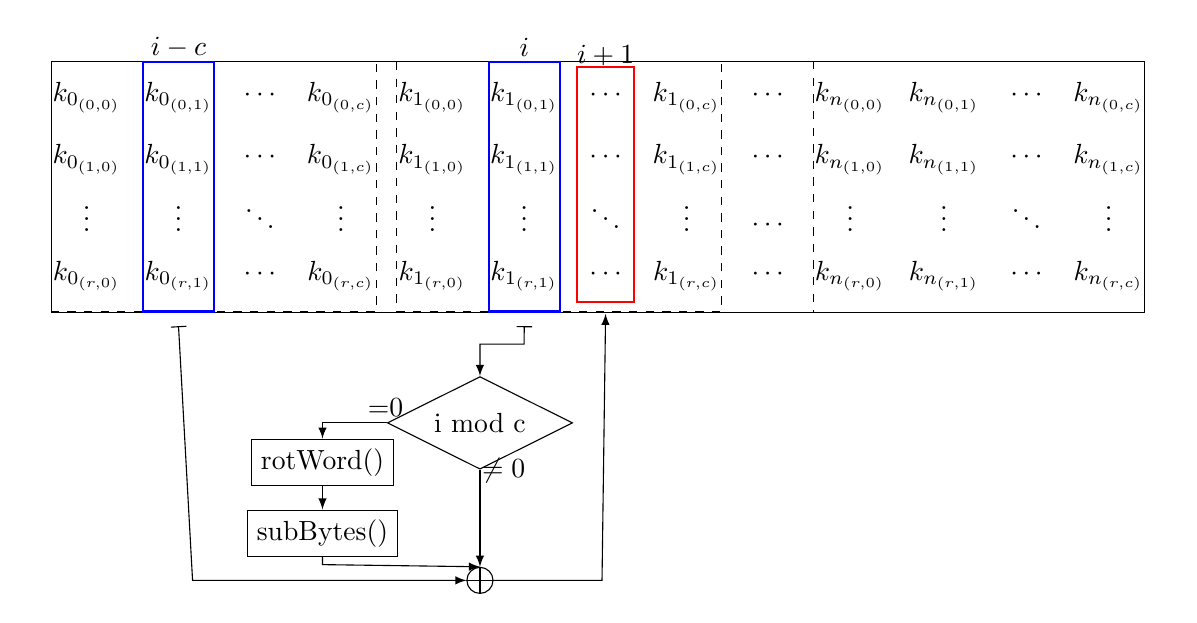
\begin{tikzpicture}[>=latex]
\matrix (k) [matrix of math nodes,nodes = {node style ge},%
              %left delimiter  = (,right delimiter = ),
              column sep=-0.1cm,row sep=-0.5cm,
             ] at (0,0)
        {
          k_{0_{(0,0)}} & k_{0_{(0,1)}} & \cdots & k_{0_{(0,c)}} &
          k_{1_{(0,0)}} & k_{1_{(0,1)}} & \cdots & k_{1_{(0,c)}} &
          \cdots &
          k_{n_{(0,0)}} & k_{n_{(0,1)}} & \cdots & k_{n_{(0,c)}} \\
          k_{0_{(1,0)}} & k_{0_{(1,1)}} & \cdots & k_{0_{(1,c)}} &
          k_{1_{(1,0)}} & k_{1_{(1,1)}} & \cdots & k_{1_{(1,c)}} &
          \cdots &
          k_{n_{(1,0)}} & k_{n_{(1,1)}} & \cdots & k_{n_{(1,c)}} \\
          \vdots        & \vdots        & \ddots & \vdots        &
          \vdots        & \vdots        & \ddots & \vdots        &
          \cdots        &
          \vdots        & \vdots        & \ddots & \vdots        \\
          k_{0_{(r,0)}} & k_{0_{(r,1)}} & \cdots & k_{0_{(r,c)}} &
          k_{1_{(r,0)}} & k_{1_{(r,1)}} & \cdots & k_{1_{(r,c)}} &
          \cdots &
          k_{n_{(r,0)}} & k_{n_{(r,1)}} & \cdots & k_{n_{(r,c)}}\\
        };
\draw [] (k-1-1.north west) rectangle (k-4-13.south east);
\draw [dashed] (k-1-1.north west) rectangle (k-4-4.south east);
\draw [dashed] (k-1-5.north west) rectangle (k-4-8.south east);
\draw [dashed] (k-1-10.north west) rectangle (k-4-13.south east);

%boxes to get the necessary columns
\draw [blue,thick] (k-1-2.north west) rectangle (k-4-2.south east);
\draw [blue,thick] (k-1-6.north west) rectangle (k-4-6.south east);
\draw [red,thick] (k-1-7.north west) rectangle (k-4-7.south east);
% 
\node [diamond,draw,aspect=2] (imodc) at (-1.5,-3) {i mod c};
\node [rectangle,draw] (rotWord) at (-3.5,-3.5) {rotWord()};
\node [rectangle,draw] (subBytes) at (-3.5,-4.4) {subBytes()};
\node [circle,draw] (xor) at (-1.5,-5) {};
 \draw [-] (xor.north) -- (xor.south);
 \draw [-] (xor.west) -- (xor.east);
\node [] (eq0) at (-2.7,-2.8) {=0};
\node [] (neq) at (-1.2,-3.6) {$\neq0$};
\node [] (neq) at (k-1-2.north) {$i-c$};
\node [] (neq) at (k-1-6.north) {$i$};
\node [] (neq) at (k-1-7.north) {$i+1$};
% 
% %arrows to set into the algorithm
\draw [|->] (k-4-2.south) -- (-5.15,-5) -- (xor.west);
\draw [|->] (k-4-6.south) -- (-.94,-2) -- (-1.5,-2) -- (imodc);
\draw [->] (imodc.west) -- (-3.5,-3) -- (rotWord.north);
\draw [->] (rotWord.south) -- (subBytes.north);
\draw [->] (imodc.south) -- (xor.north);
\draw [->] (subBytes.south) -- (-3.5,-4.8) -- (xor.north);
\draw [->] (xor.east) -- (0.05,-5) -- (k-4-7.south);

\end{tikzpicture}
\caption{Block diagram of the iterative construction of the \emph{Rijndael Key Expansion} as a \emph{PseudoRandomGenerator}, PRG}
\label{fig:keyExpansionDiagram}
\end{center}
\end{figure}



%%%%%%%%%%%%%%%%
\subsection{Rounds}
% TODO why n rounds and not more, not less?

%%%%%%%%%%%%%%%%
\subsection{subBytes}
This transformation is a non-linear substitution of each word in the \emph{state} matrix. In the original Rijndael it is used a substitution table called \emph{S-Box}. This S-Box is represented in the figure \ref{tab:sbox8} and there is also an inverse of it.

\begin{figure}[b]{\tiny
\begin{center}
\begin{tabular}[]{|l||l|l|l|l|l|l|l|l|l|l|l|l|l|l|l|l|}\hline
    & 0x0  & 0x1  & 0x2  & 0x3  & 0x4  & 0x5  & 0x6  & 0x7  & 0x8  & 0x9  & 0xA  & 0xB  & 0xC  & 0xD  & 0xE  & 0xF \\\hline\hline
0x0 & 0x63 & 0x7C & 0x77 & 0x7B & 0xF2 & 0x6B & 0x6F & 0xC5 & 0x30 & 0x01 & 0x67 & 0x2B & 0xFE & 0xD7 & 0xAB & 0x76\\\hline
0x1 & 0xCA & 0x82 & 0xC9 & 0x7D & 0xFA & 0x59 & 0x47 & 0xF0 & 0xAD & 0xD4 & 0xA2 & 0xAF & 0x9C & 0xA4 & 0x72 & 0xC0 \\\hline
0x2 & 0xB7 & 0xFD & 0x93 & 0x26 & 0x36 & 0x3F & 0xF7 & 0xCC & 0x34 & 0xA5 & 0xE5 & 0xF1 & 0x71 & 0xD8 & 0x31 & 0x15 \\\hline
0x3 & 0x04 & 0xC7 & 0x23 & 0xC3 & 0x18 & 0x96 & 0x05 & 0x9A & 0x07 & 0x12 & 0x80 & 0xE2 & 0xEB & 0x27 & 0xB2 & 0x75 \\\hline
0x4 & 0x09 & 0x83 & 0x2C & 0x1A & 0x1B & 0x6E & 0x5A & 0xA0 & 0x52 & 0x3B & 0xD6 & 0xB3 & 0x29 & 0xE3 & 0x2F & 0x84 \\\hline
0x5 & 0x53 & 0xD1 & 0x00 & 0xED & 0x20 & 0xFC & 0xB1 & 0x5B & 0x6A & 0xCB & 0xBE & 0x39 & 0x4A & 0x4C & 0x58 & 0xCF \\\hline
0x6 & 0xD0 & 0xEF & 0xAA & 0xFB & 0x43 & 0x4D & 0x33 & 0x85 & 0x45 & 0xF9 & 0x02 & 0x7F & 0x50 & 0x3C & 0x9F & 0xA8 \\\hline
0x7 & 0x51 & 0xA3 & 0x40 & 0x8F & 0x92 & 0x9D & 0x38 & 0xF5 & 0xBC & 0xB6 & 0xDA & 0x21 & 0x10 & 0xFF & 0xF3 & 0xD2 \\\hline
0x8 & 0xCD & 0x0C & 0x13 & 0xEC & 0x5F & 0x97 & 0x44 & 0x17 & 0xC4 & 0xA7 & 0x7E & 0x3D & 0x64 & 0x5D & 0x19 & 0x73 \\\hline
0x9 & 0x60 & 0x81 & 0x4F & 0xDC & 0x22 & 0x2A & 0x90 & 0x88 & 0x46 & 0xEE & 0xB8 & 0x14 & 0xDE & 0x5E & 0x0B & 0xDB \\\hline
0xA & 0xE0 & 0x32 & 0x3A & 0x0A & 0x49 & 0x06 & 0x24 & 0x5C & 0xC2 & 0xD3 & 0xAC & 0x62 & 0x91 & 0x95 & 0xE4 & 0x79 \\\hline
0xB & 0xE7 & 0xC8 & 0x37 & 0x6D & 0x8D & 0xD5 & 0x4E & 0xA9 & 0x6C & 0x56 & 0xF4 & 0xEA & 0x65 & 0x7A & 0xAE & 0x08 \\\hline
0xC & 0xBA & 0x78 & 0x25 & 0x2E & 0x1C & 0xA6 & 0xB4 & 0xC6 & 0xE8 & 0xDD & 0x74 & 0x1F & 0x4B & 0xBD & 0x8B & 0x8A \\\hline
0xD & 0x70 & 0x3E & 0xB5 & 0x66 & 0x48 & 0x03 & 0xF6 & 0x0E & 0x61 & 0x35 & 0x57 & 0xB9 & 0x86 & 0xC1 & 0x1D & 0x9E \\\hline
0xE & 0xE1 & 0xF8 & 0x98 & 0x11 & 0x69 & 0xD9 & 0x8E & 0x94 & 0x9B & 0x1E & 0x87 & 0xE9 & 0xCE & 0x55 & 0x28 & 0xDF \\\hline
0xF & 0x8C & 0xA1 & 0x89 & 0x0D & 0xBF & 0xE6 & 0x42 & 0x68 & 0x41 & 0x99 & 0x2D & 0x0F & 0xB0 & 0x54 & 0xBB & 0x16 \\\hline
\end{tabular}
\end{center}}
\caption{Sbox for 8 bits word size}
\label{tab:sbox8}
\end{figure}

From the programmatic point of view the use of those boxes is so simple. Because the wordsize is 8 bits, by splitting the data to transform in two parts of 4 bits you can get the row and the column, taking the value in the cell as the value of the substitution. In the decipher operation, is used the inverse of the box, and with the same procedure of split the word and find the coordinates, but now with the inverse S-Box, the value you get back is the original data.

As an example, to transform the data \texttt{0x39} localise the cell in row \texttt{0x3} column \texttt{0x9}, and change the state matrix value with \texttt{0x12}. In the decipher procedure the transformation will be from the value \texttt{0x12}, reading the row \texttt{0x1} column \texttt{0x2} the cell have the value \texttt{0x39}, the original of this example.

% abstraction of what it is, independent from the #rows, #columns, wordsize

But this tool of the \emph{S-Box} is a faster way to compose two transformations in one and with not much computation.

% operations in the polynomial field F_{2^w} w: wordsize
The first transformation is to compute the multiplicative inverse in the field \Fpn{2}{w}, where w is the wordsize ($w=8$ in the original Rijndael). The second transformation is an affine transformation over the field \Fpn{2}{w}. In the original Rijndael is:
\begin{equation}\label{eq:subBytes:affine}
 b_{i}' = b_{i} \oplus b_{(i+4)mod8} \oplus b_{(i+5)mod8} \oplus 
          b_{(i+6)mod8} \oplus b_{(i+7)mod8} \oplus c_{i}
\end{equation}
Where $b$ is the byte to be transformed and $c$ is a fix value \texttt{0x63=0b01100011}. This transformation can be expressed as a matrix operation:

\begin{equation}
 \left[
  \begin{array}{c}
    b_{0}'\\b_{1}'\\b_{2}'\\b_{3}'\\b_{4}'\\b_{5}'\\b_{6}'\\b_{7}'
  \end{array}
 \right]=\left[
  \begin{array}{cccccccc}
    1&0&0&0&1&1&1&1\\
    1&1&0&0&0&1&1&1\\
    1&1&1&0&0&0&1&1\\
    1&1&1&1&0&0&0&1\\
    1&1&1&1&1&0&0&0\\
    0&1&1&1&1&1&0&0\\
    0&0&1&1&1&1&1&0\\
    0&0&0&1&1&1&1&1\\
  \end{array}
 \right]\cdot\left[
  \begin{array}{c}
    b_{0}\\b_{1}\\b_{2}\\b_{3}\\b_{4}\\b_{5}\\b_{6}\\b_{7}
  \end{array}
 \right]+\left[
  \begin{array}{c}
    1\\1\\0\\0\\0\\1\\1\\0
  \end{array}
 \right]
\end{equation}

% TODO draw schematic of this step

%%%%%%%%%%%%%%%%
\subsubsection{How to build different SBoxes}

% TODO and how to build a new one with different parameters
Using the same \emph{wordsize} there are two different things that can be changed: the \texttt{0x63} and the product over the field of equation \ref{eq:subBytes:affine}. If the option is to use another wordsize this is the unique main parameter of the original Rijndael to set a different. With a wordsize of $4$ the operations will be defined over \Fpn{2}{4}, over $16$ the field will be \Fpn{2}{{16}}, and the subparameters of the affine transformation must also be set up.

%%%%%%%%%%%%%%%%
\subsection{shiftColumns}
% TODO abstraction of what it is, independent from the #rows,GeneralizedRijndael/sboxes.py #columns, wordsize
% FIXME(review) draw schematic of this step
\begin{figure}
\begin{center}
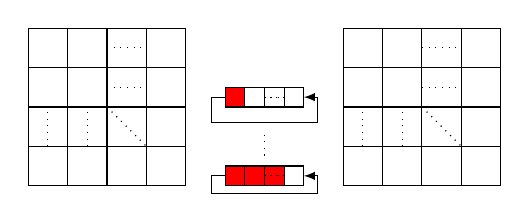
\begin{tikzpicture}[>=latex]
 
%  \matrix (k) [matrix of math nodes,nodes = {node style ge},%
%               %left delimiter  = (,right delimiter = ),
%               column sep=-0.1cm,row sep=-0.5cm,
%              ] at (0,0)
%         {
%           s_{(0,0)} & s_{(0,1)} & \cdots & s_{(0,c)} \\
%           s_{(1,0)} & s_{(1,1)} & \cdots & s_{(1,c)} \\
%           \vdots    & \vdots    & \ddots & \vdots    \\
%           s_{(r,0)} & s_{(r,1)} & \cdots & s_{(r,c)} \\
%         };

\draw (0.0,0.0) rectangle (2.0,0.5);
\draw (0.0,0.5) rectangle (2.0,1.0);
\draw (0.0,1.0) rectangle (2.0,1.5);
\draw (0.0,1.5) rectangle (2.0,2.0);
\draw (0.5,0.0) rectangle (1.0,2.0);
\draw (1.5,0.0) rectangle (2.0,2.0);
\draw [dotted] (0.25,0.50) -- (0.25,1.0);
\draw [dotted] (0.75,0.50) -- (0.75,1.0);
\draw [dotted] (1.00,1.00) -- (1.50,0.50);
\draw [dotted] (1.00,1.25) -- (1.50,1.25);
\draw [dotted] (1.00,1.75) -- (1.50,1.75);

\draw [fill=red] (2.50,1.0) rectangle (2.75,1.25);
\draw (2.75,1.0) rectangle (3.00,1.25);
\draw (3.00,1.0) rectangle (3.25,1.25);
\draw (3.25,1.0) rectangle (3.50,1.25);
\draw [->] (2.500,1.125)--(2.325,1.125)--(2.325,0.80)--(3.675,0.80)--(3.675,1.125)--(3.50,1.125);
\draw [dotted] (3.0,1.125) rectangle (3.25,1.125);

\draw [dotted] (3.00,0.65) -- (3.00,0.35);

\draw [fill=red] (2.50,0.0) rectangle (2.75,0.25);
\draw [fill=red] (2.75,0.0) rectangle (3.00,0.25);
\draw [fill=red] (3.00,0.0) rectangle (3.25,0.25);
\draw (3.25,0.0) rectangle (3.50,0.25);
\draw [->] (2.500,0.125)--(2.325,0.125)--(2.325,-0.10)--(3.675,-0.10)--(3.675,0.125)--(3.50,0.125);
\draw [dotted] (3.00,0.125) rectangle (3.25,0.125);

\draw (4.0,0.0) rectangle (6.0,0.5);
\draw (4.0,0.5) rectangle (6.0,1.0);
\draw (4.0,1.0) rectangle (6.0,1.5);
\draw (4.0,1.5) rectangle (6.0,2.0);
\draw (4.5,0.0) rectangle (5.0,2.0);
\draw (5.5,0.0) rectangle (6.0,2.0);
\draw [dotted] (4.25,0.50) -- (4.25,1.0);
\draw [dotted] (4.75,0.50) -- (4.75,1.0);
\draw [dotted] (5.00,1.00) -- (5.50,0.50);
\draw [dotted] (5.00,1.25) -- (5.50,1.25);
\draw [dotted] (5.00,1.75) -- (5.50,1.75);


\end{tikzpicture}
\caption{Schematic diagram of the shiftColumns() transformation}
\label{fig:shiftColumns}
\end{center}
\end{figure}


%%%%%%%%%%%%%%%%
\subsection{mixColumns}
% TODO abstraction of what it is, independent from the #rows, #columns, wordsize
% TODO polynomial ring, where the coeficients are elements from a binary polynomial field
%   \Fpnm{x}{z}, ord(m)=#rows
%   (this is, in mho, one of the most important points of rijndael)
% FIXME (review) draw schematic of this step

\begin{figure}
\begin{center}
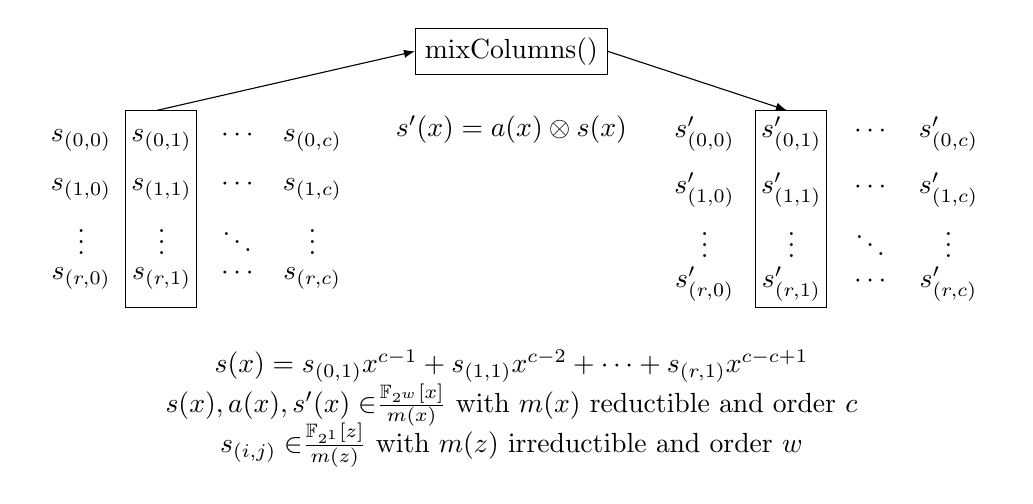
\begin{tikzpicture}[>=latex]
 
 \matrix (s) [matrix of math nodes,nodes = {node style ge},%
              %left delimiter  = (,right delimiter = ),
              column sep=-0.1cm,row sep=-0.5cm,
             ] at (-4,0)
        {
          s_{(0,0)} & s_{(0,1)} & \cdots & s_{(0,c)} \\
          s_{(1,0)} & s_{(1,1)} & \cdots & s_{(1,c)} \\
          \vdots    & \vdots    & \ddots & \vdots    \\
          s_{(r,0)} & s_{(r,1)} & \cdots & s_{(r,c)} \\
        };

\draw (-4.9,1.25)rectangle(-4,-1.25);

 \matrix (s') [matrix of math nodes,nodes = {node style ge},%
              %left delimiter  = (,right delimiter = ),
              column sep=-0.1cm,row sep=-0.5cm,
             ] at (4,0)
        {
          s'_{(0,0)} & s'_{(0,1)} & \cdots & s'_{(0,c)} \\
          s'_{(1,0)} & s'_{(1,1)} & \cdots & s'_{(1,c)} \\
          \vdots    & \vdots    & \ddots & \vdots    \\
          s'_{(r,0)} & s'_{(r,1)} & \cdots & s'_{(r,c)} \\
        };
\draw (3.1,1.25)rectangle(4,-1.25);

\node [rectangle,draw] (mixColumns) at (0,2) {mixColumns()};
 \draw [->] (-4.5,1.25)--(mixColumns.west);
 \draw [->] (mixColumns.east)--(3.5,1.25);

\node [rectangle] (poli) at (0,1.0) {$s'(x)=a(x)\otimes s(x)$};
\node [rectangle] (sx) at (0,-2) {$s(x)=s_{(0,1)}x^{c-1}+s_{(1,1)}x^{c-2}+\cdots+s_{(r,1)}x^{c-c+1}$};
\node [rectangle] (fpnm) at (0,-2.5) {$ s(x),a(x),s'(x) \in$\Fpnm{w}{x} with $m(x)$ reductible and order $c$};
\node [rectangle] (fpn) at (0,-3) {$s_{(i,j)} \in$\Fpnm{1}{z} with $m(z)$ irreductible and order $w$};

\end{tikzpicture}
\caption{Diagram of the mixColumns() operation over the polynomial ring with coeficients in a polynomial field}
\label{fig:mixColumns}
\end{center}
\end{figure}


\subsection{Operate in a polinomial ring, with coeficients in a polinomial field}
$$\Fpnm{n}{y}\label{eq:polinomialRing}$$ where $m(y)$ is a composed polinomial of degree $r$ columns. This gives a polinomial ring. The coeficients of this polinomial ring are elements of a polinomial field $$\Fpn{2}{n}=\Fpnm{2}{x}\label{eq:polinomialField}$$ where $m(x)$ is irreductible and gives a polinomial field.
Standard rijndael (AES) uses a circulan invertible matrix for this to simplify and speed up the operations in the ring.

%%%%%%%%%%%%%%%%
\subsection{addRoundKey}
% TODO the operation where the key is used (from the 4 rijndael operations)
% TODO simply a xor operation (addition in F_2)
% TODO draw schematic of this step

%%%%%%%%%%%%%%%%
\section{Parameter combinations}
% TODO how, with different parameters, can have the same block sizes, and what's different between them

%%%%%%%%%%%%%%%%
\section{New useful sizes for Rijndael}
% TODO because of the newer processors with 64 bits, it can be easy to have bigger sizes with less costs
\cite{Daemen:1999:EBC:1267115.1267119}

%%%%%%%%%%%%%%%%
%TODO: what else should be in the paper?
% \section{Attacking the schema}
% 
% \subsection{Side channel attacks}
% %?difference between precalculated sbox and rcon or compute on the fly
% % constant time operation intervals and equivalent memory use
% % key expansion calculated during the encrypt/decrypt process
% \section{Conclusions}

%%%%%%%%%%%%%%%%
\bibliographystyle{ieeetr}
\bibliography{../bibtex/sblanch.bib,../bibtex/standards.bib,../bibtex/symmetrics.bib,../bibtex/rijndael.bib,../bibtex/books.bib,../bibtex/crypto.bib,../bibtex/rfc.bib}

\end{document}